% Project 1 - EECS 499
% Authors: Shaun Howard and Matt Swartwout
\documentclass[conference]{IEEEtran}
\usepackage[T1]{fontenc}
\usepackage[backend=biber, style=ieee]{biblatex}
\addbibresource{report.bib}
\usepackage[final]{microtype}
%\usepackage{appendix}
\usepackage{listings}

% *** GRAPHICS RELATED PACKAGES ***
%
\ifCLASSINFOpdf
  \usepackage[pdftex]{graphicx}
  % declare the path(s) where your graphic files are
  \graphicspath{{images/}}
  % and their extensions so you won't have to specify these with
  % every instance of \includegraphics
  \DeclareGraphicsExtensions{.jpeg,.png}
\else
  % or other class option (dvipsone, dvipdf, if not using dvips). graphicx
  % will default to the driver specified in the system graphics.cfg if no
  % driver is specified.
  % \usepackage[dvips]{graphicx}
  % declare the path(s) where your graphic files are
  % \graphicspath{{../eps/}}
  % and their extensions so you won't have to specify these with
  % every instance of \includegraphics
  % \DeclareGraphicsExtensions{.eps}
\fi
% graphicx was written by David Carlisle and Sebastian Rahtz. It is
% required if you want graphics, photos, etc. graphicx.sty is already
% installed on most LaTeX systems. The latest version and documentation
% can be obtained at: 
% http://www.ctan.org/pkg/graphicx
% Another good source of documentation is "Using Imported Graphics in
% LaTeX2e" by Keith Reckdahl which can be found at:
% http://www.ctan.org/pkg/epslatex
%
% latex, and pdflatex in dvi mode, support graphics in encapsulated
% postscript (.eps) format. pdflatex in pdf mode supports graphics
% in .pdf, .jpeg, .png and .mps (metapost) formats. Users should ensure
% that all non-photo figures use a vector format (.eps, .pdf, .mps) and
% not a bitmapped formats (.jpeg, .png). The IEEE frowns on bitmapped formats
% which can result in "jaggedy"/blurry rendering of lines and letters as
% well as large increases in file sizes.
%
% You can find documentation about the pdfTeX application at:
% http://www.tug.org/applications/pdftex

% correct bad hyphenation here
\hyphenation{op-tical net-works semi-conduc-tor}


\begin{document}

% paper title
% Titles are generally capitalized except for words such as a, an, and, as,
% at, but, by, for, in, nor, of, on, or, the, to and up, which are usually
% not capitalized unless they are the first or last word of the title.
% Linebreaks \\ can be used within to get better formatting as desired.
% Do not put math or special symbols in the title.
\title{Distributed State Estimation in a 1-D World}


% author names and affiliations
% use a multiple column layout for up to three different
% affiliations
\author{
\IEEEauthorblockN{Shaun Howard \ \ Matt Swartwout}
\IEEEauthorblockA{Electrical Engineering and Computer Science Department\\
Case Western Reserve University\\
Cleveland, Ohio 44106\\
Email: \{smh150, mws85\}@case.edu}
}

% make the title area
\maketitle

% As a general rule, do not put math, special symbols or citations
% in the abstract
\begin{abstract}
In this paper, we propose the use of both an Extended Kalman Filter (EKF) and an Unscented Kalman Filter (UKF) in order 
to determine the x-position of a single mobile robot (R) given multiple noisy sensor measurements. Given a squadron of 
N robots in a one-dimensional environment, the x-position of robot R with noisy odometry data can be estimated via the 
sensor measurements of all N robots denoted S. Each robot in S can monitor the true position of R via their laser scan 
sensor in order to build a set of pose estimates for R. The resulting set of N-1 pose estimates can be filtered in a 
distributed fashion either via an EKF or UKF in order to accurately estimate the current pose of R in the 
one-dimensional environment.

We demonstrate the usefulness of this state estimation procedure through a three robot simulation in Gazebo. We compare 
the results of the distributed filter with a self-filter in this environment where R estimates its own position via 
object detection and either an EKF or UKF. We simulate the use of each filter with varying speeds of R. We analyze and 
compare filter results from each simulation in order to determine the reliability of each filter. Our simulation 
results reveal that the distributed filter frequently out-performs the self-filter in terms of accuracy without any 
additional parameter tuning.
\end{abstract}
% Same thing here, we didn't actually look into attacking any sensors
The idea behind the method is derived from the method proposed in [1]. Their method uses an EKF to predict the
position of one terrorized robot given N sensor measurements. The difference between the methods is that this
method analyses the usage of an EKF as well as UKF for estimating the position of a terrorized robot
given N-1 measurements from remote sensors and a single sensor measurement given point cloud data from the affected robot.
Both filters show remarkable results in tracking the terrorized robot's position over time, but the UKF beats the EKF in accuracy most of the time. The simulation uses three robots with one terrorized and monitored by the other two to test the estimation hypothesis and prove that UKF works with one-dimensional robot position estimation from N noisy sensor measurements.

% start of introduction
\section{Introduction}

% write brief history
Autonomous mobile robotic systems have gained prevalence in the past 10 years. Along with this
growth in usage, terrorist attacks have become more frequent on such systems.
Many current autonomous mobile robot systems are prone to attack given the wireless interfaces present
on the robots in order to send and receive communications from a command base. Increased attention has
been given to this area in recent years, but many methods still fail to recognize that a chain of robots
maybe become terrorized at once.
\par
% write issue areas and reasons to do our research
Not only do robots have to deal with noise from their sensors, but they also are prone to loss of communications
with their remote global positioning systems (GPS). As demonstrated in [2], terrorists use a spoofed GPS system
to knock a yacht off course. Terrorist attacks are a growing threat that must be addressed in order to save
valuable robotic systems from danger zones. Figure 1 displays three TurtleBots in the Gazebo simulator world. The middle TurtleBot is the terrorized robot that moves back and forth between the other two, safe robots which monitor it as it moves. As the middle robot undergoes attack, the proposed system should provide the terrorized robot with a reasonable position estimation for safe navigational purposes such as avoiding danger zones in an environment or on a map.
\par 
% discuss image and experimental/sim setup
Figure 1 is a reference for the simulation experiments performed in this paper. The proposed method takes
interest in estimating the state of the moving terrorized robot according to the distances between the robots acquired through point cloud scans of all the robots.
\par
\begin{figure}[!ht]
  \centering
    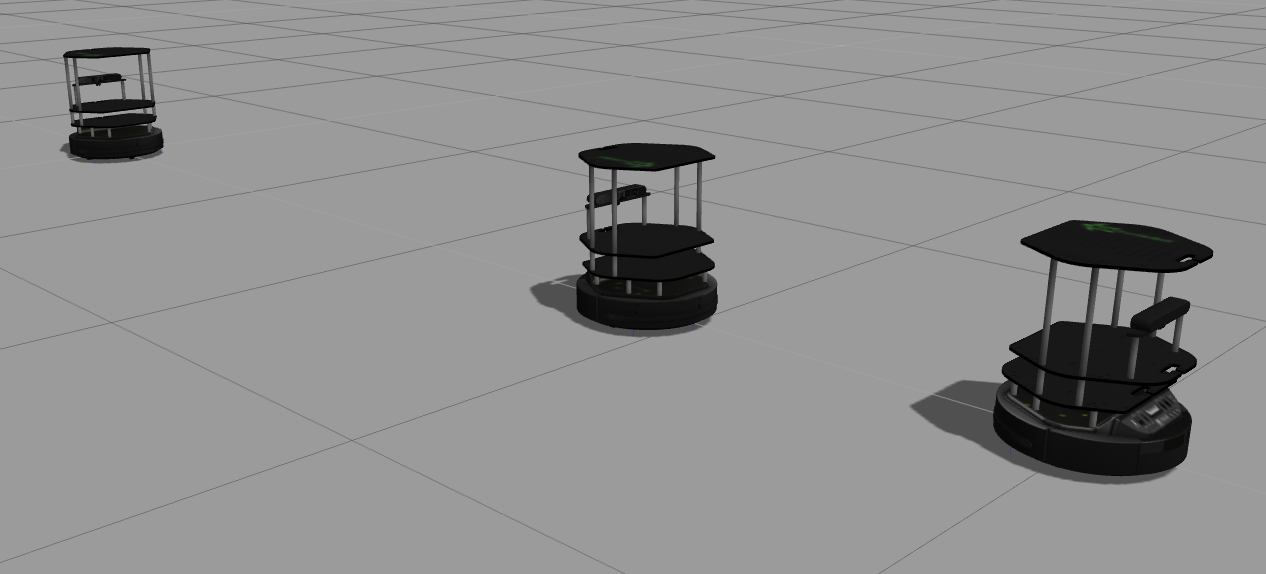
\includegraphics[scale=.2]{sim1}
  \caption{Three TurtleBots on a world-based grid world attempt to estimate the position of the moving and terrorized robot.}
\end{figure}
\par
Importantly, redundancy is considered by utilizing N-1 sensor readings from other robots in addition to the
sensor on the moving robot in order to estimate the state of moving robot in the world. Problems such as the one posed in this paper can be solved by EKFs and UKFs. EKFs can be applied to many other cyber-physical systems that utilize multiple sensor measurements to make a prediction about the position a system.
\par
% discuss method using EKF and UKF
This paper contributes (1) slight modifications to the ROMDP algorithm proposed in [1], (2) a proposed technique
to deal with up to N-1 terrorized robots each with sensors measuring their own and other robot locations
using ROMDP paired with a particle filter, and (3) simulation and experimental results important to evaluate
the usability of this method in real-world scenarios considering mobile robots with monitoring allies.
\par
% discuss paper organization
Following, the paper is organized like so: Section 2 describes work related to the method proposed; Section 3
formally defines the problem being investigated; Section 4.1 covers the details the ROMDP algorithm and any
modifications made; Section 4.2 details the generic particle filter algorithm; Section 4.3 outlines the positional
state estimation technique proposed using ROMDP and the generic particle filter; Section 5 covers the
simulation outline, process and experimental results of a robot with terrorized sensors and 2 non-terrorized
co-operatives. Lastly, section 6 concludes the paper and future work is discussed.
% end of introduction

% start of related work
\section{Related Work}

% end of related work

% start of problem
\section{Problem Formulation}
% This should probably go in the introduction somewhere
The concept of sensor fusion and combining multiple sensor readings within a single robot has been well shown.
By combining data from multiple sensors and feeding that information into an EKF or UKF, the total accuracy of the
system can be improved.
Inherent noise in one sensor will propagate less into the final result, and the loss of a single or multiple sensors
will not necessarily result in catastrophic failure of the system.

Our problem specification is created from these core tenets:
\begin{enumerate}
\item A finite 1-D system containing a mobile robot
\item A physical landmark (e.g. stationary robot) at each end of the system
\item The mobile robot and landmarks are all equipped with a sensor that measures distance
\item The mobile robot can move forwards and backwards, but cannot change its orientation (this obviates the need for a
recognition system between the robot and landmarks)
\end{enumerate}

The core problems solved in the implementation of this system are:
\begin{enumerate}
\item Implementation of Extended and Unscented Kalman filters via the robot\_localization package
\cite{robot_localization}
\item Create a ROS \cite{ros_original} system that simulates a TurtleBot 2 and the stationary landmarks in Gazebo
\cite{gazebo}.
\item Create a ROS node system for the Turtlebot 2 that facilitates communication between the mobile robot and the 
stationary landmarks, and also transforms and feeds those measurements into the filters.
\end{enumerate}
% end of problem


% start robot predict
\section{Methodology}
As stated above, the project naturally divided itself into three main problems. These three problems were the
implementation of the Extended and Unscented Kalman filters, simulation of the Turtlebot 2 and 1-D environment in 
Gazebo, and creating the system of ROS nodes for the Turtlebot 2 to communicate with the stationary landmarks and the 
filters.

\subsection{Filter Implementation}
We chose to implement our filters using the previously mentioned robot\_localization. We chose this package due to its 
ability to do sensor fusion of an arbitrary number of sensors, because it was built for ROS, and because of the simple 
setup but also the complex configurations that it enables.

We implemented both an Extended and Unscented Kalman filter, but the actual configuration parameters for both of them 
were identical. Additionally, we implemented two filters on the mobile robot. The first we called the "Self" filter, 
and used only one distance measurements, taken by the robot's distance sensor to the landmark directly in front of it. 
The second filter we called the "Distributed" filter, and it took measurements from the robot's sensor, and also both 
of the landmark's sensors. All measurements were fed to the filter as a geometry\_msgs/PoseWithCovarianceStamped 
messages.

For both filters we set two\_d\_mode to true, because we did not care about any 3-dimensional motion. For the first 
sensor measurement, we fused the x and y position and yaw into the final state estimate. Even though we assume a 1-D 
system with no y movement possible, and also assume that no yaw rotations will ever be made, the filters do not support 
a 1-D world so we had to include the y and yaw measurements. For the second and third sensor on the Distributed filter, 
we fused only the x position.

We also set the differential parameter to true for all sensors. This makes the filter differentiate the absolute 
position measurements received and input them as velocities rather than positions. This had two distinct advantages for 
our system. First, we did not need to worry about transforming the poses from the reference frame of the landmark to 
the reference frame of the mobile robot. Since we knew the starting position of the robot we did not need the absolute 
position measurements. Second, this reduced the error from our measurement system. The system we used was a Kinect 
camera, and we took a slice of points from its depth cloud and used this to simulate a LIDAR. Because of this, we were 
not measuring a specific, known point on the robot. Instead, we measured many points and then took the median of those 
points and represented that as the distance to the robot. By using the velocities rather than positions we mitigated 
some of the error that may have come from the median point of the scan on the robot being in slightly different 
positions from scan to scan. While error there may have existed, it would not lead to discrete jumps like the position 
measurement would have.

\subsection{Gazebo Simulation}
Our simulation experiments were run with three robots, two at fixed positions and one moving randomly between the two. 
During each experiment, R moved randomly in the x-direction at a chosen experimental speed. During each simulation 
experiment, both a distributed filter and a self-filter were utilized to approximate the x-position of R. 
The distributed filter used three pose estimates from the three robots while the self-filter mechanism used object 
detection to form a single pose estimate. Experiments were run for both distributed and self-filters simultaneously 
based on the choice of EKF or UKF. Two speeds of 0.2 m/s and 0.4 m/s were chosen during experimentation for each filter 
type in order to determine the performance of filters at various speeds in the one-dimensional environment.
\subsection{Inter-Node Communication System}

\section{Results}
% discuss and display sim vs filtered odom using std dev error bars
Figure 2 displays a comparison of the predicted odometry measurements via distributed and self filters with the actual 
simulator odometry measurements per the four experiments performed. In accordance with the figure, we observe that the 
filtered odometry is very close in accuracy to the simulator odometry in both cases.

% discuss, compare and display self and dist filtering errors vs sim odom
 Comparing both filtering approaches, we observe that the distributed filter almost always out-performs the self-filter 
 with both filter types.

% discuss, compare and display dist filters with each other based on errors from sim odom
Additionally, by no surprise we find that the UKF distributed filtering method out-performs the EKF distributed 
filtering method. Figure 4 displays the comparison in error over time of both distributed filters per experiment.

Overall, the results of our simulation support our hypothesis about the application of an EKF or UKF to accurately 
estimate the position of a single mobile robot R via N-1 other robots monitoring R in a 1-D environment. 
\section{Conclusion}
The conclusion goes here.

% use section* for acknowledgment
\section*{Acknowledgement}


The authors would like to thank...


% references section

% can use a bibliography generated by BibTeX as a .bbl file
% BibTeX documentation can be easily obtained at:
% http://mirror.ctan.org/biblio/bibtex/contrib/doc/
% The IEEEtran BibTeX style support page is at:
% http://www.michaelshell.org/tex/ieeetran/bibtex/
%\bibliographystyle{IEEEtran}
% argument is your BibTeX string definitions and bibliography database(s)
%\bibliography{IEEEabrv,../bib/paper}
%
% <OR> manually copy in the resultant .bbl file
% set second argument of \begin to the number of references
% (used to reserve space for the reference number labels box)

\printbibliography




% that's all folks
\end{document}